
\documentclass[11pt,serif,aspectratio=169]{beamer}

% Set the margins to be something normal.
% \usepackage[margin=1in]{geometry}

% Fun lists!
\usepackage{enumitem}
\usepackage{textcomp}
\setitemize{label=\textrightarrow, itemsep=0pt}

% Math symbols.
\usepackage{amsmath, amssymb, amsfonts, tikz,mathtools}

% No indents.
\setlength\parindent{0pt}
\setlength\parskip{1em}

\newcommand{\inverse}[1]{#1^{-1}}


% Nice fonts :)
%\usepackage{tgschola}
\usefonttheme[onlymath]{serif}

\begin{document}
	\begin{frame}[c]\centering \Large \bf
		Euler's identity and hyperbolic functions	
	\end{frame}
	
	\begin{frame}[c]
		\textbf{Polar coordinates} tell us where something is using an \textbf{angle from the origin} and a \textbf{stretching factor}.
	\end{frame}
	
	\begin{frame}[c]
		\begin{figure}
			\centering
			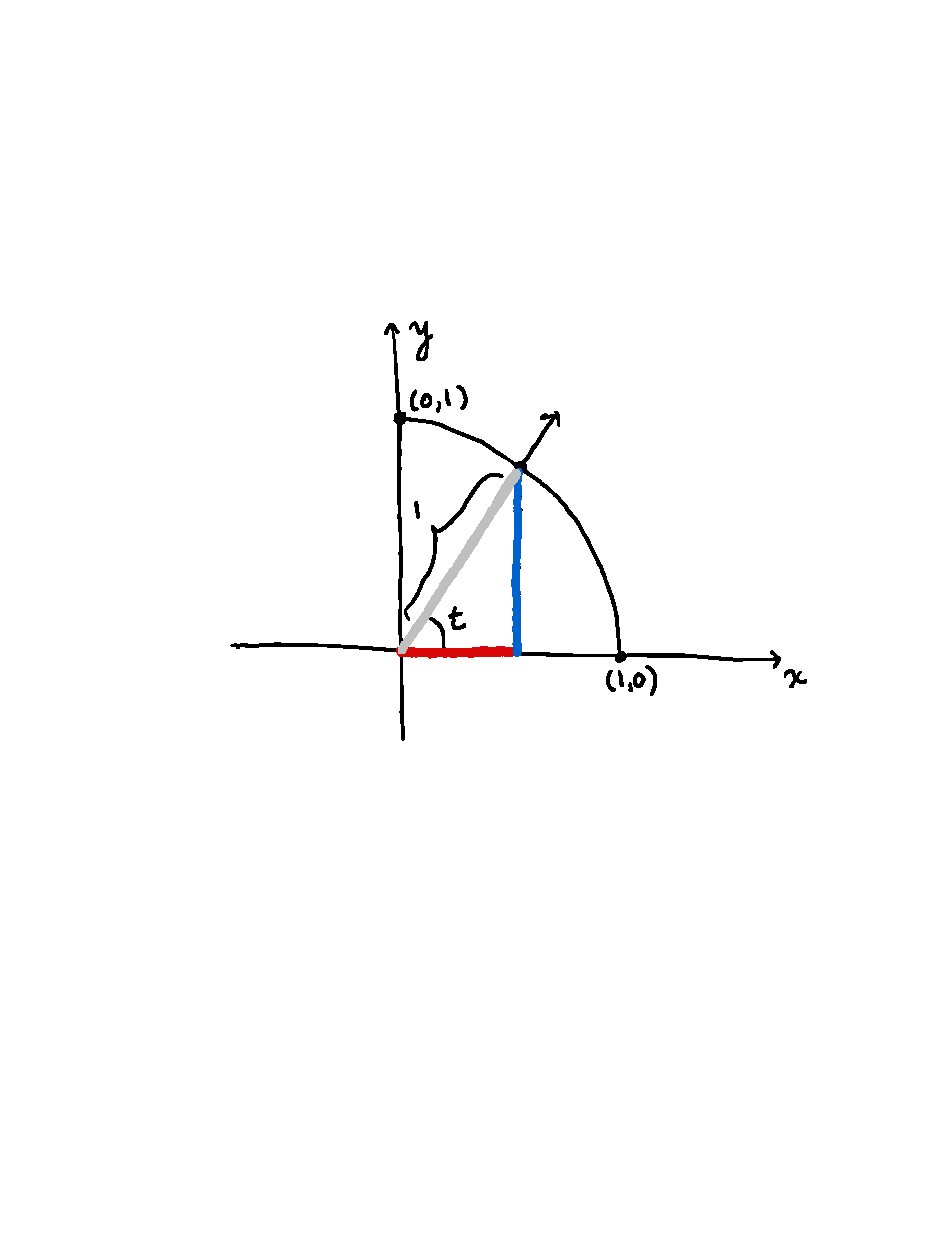
\includegraphics[height=0.9\paperheight]{polar.pdf}	
		\end{figure}
	\end{frame}
	
	\begin{frame}[c]
		\begin{figure}
			\centering
			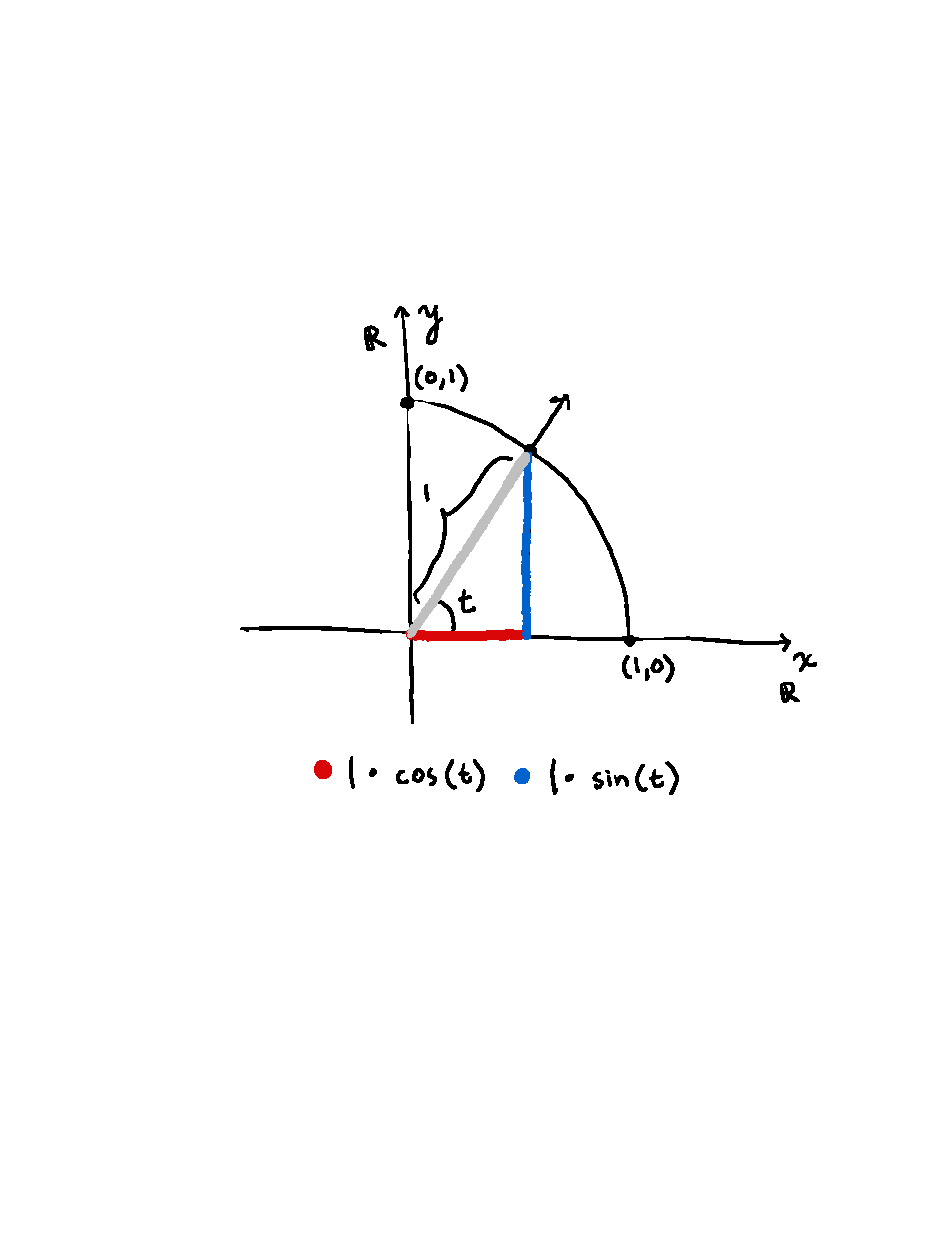
\includegraphics[height=0.9\paperheight]{polar-with-trig.pdf}	
		\end{figure}
	\end{frame}
	
	\begin{frame}[c]
		Because complex numbers are written as $$ a + bi,$$ with $a$ a real number and $b$ a stretching (scaling) factor on the complex number $i$, we can say that \begin{center} $a$ represents \textbf{stretching in the $x$ direction}\end{center} and \begin{center} $bi$ represents \textbf{stretching in the $i$ direction}.\end{center}
	\end{frame}
	
	\begin{frame}[c]
		\begin{figure}
			\centering
			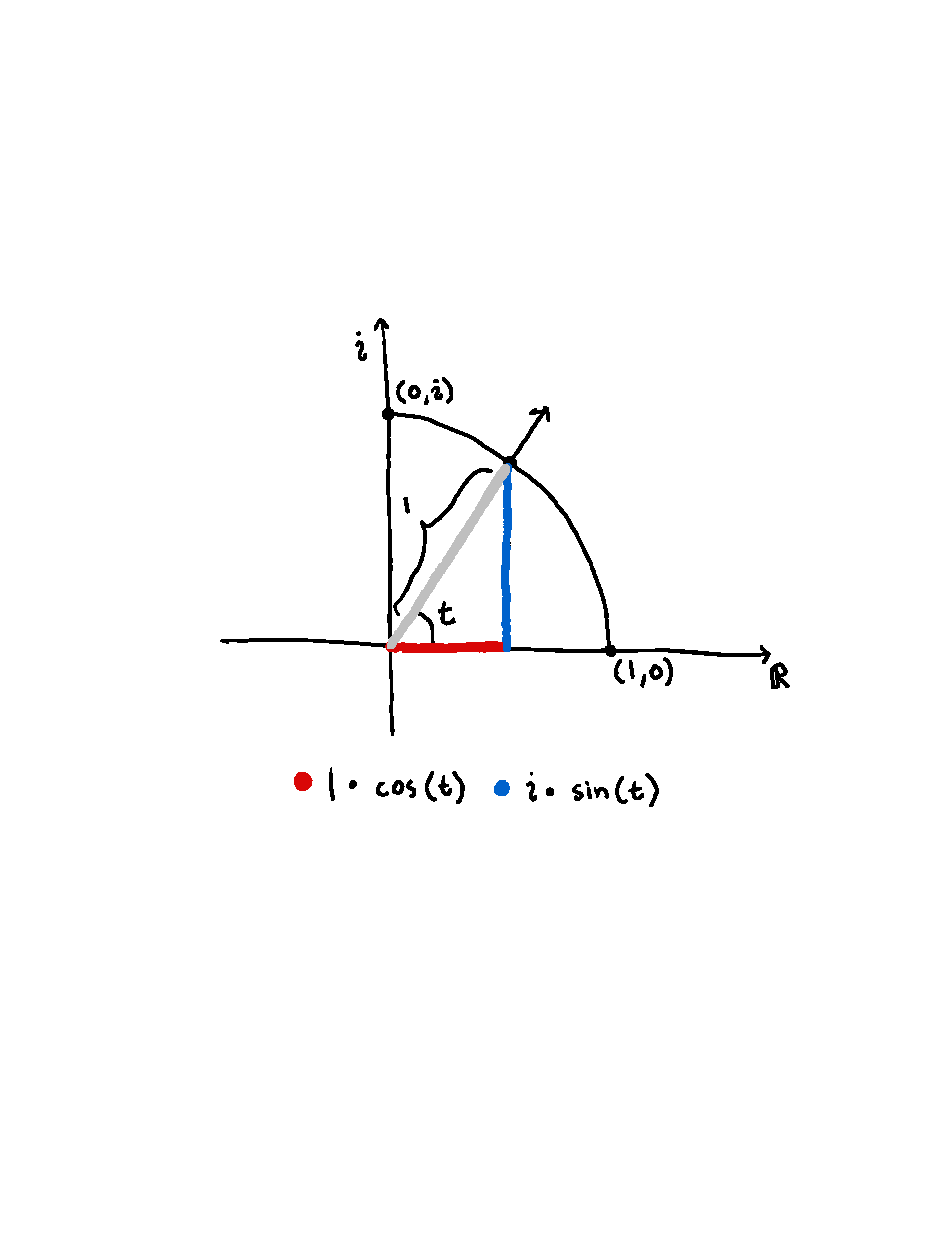
\includegraphics[height=0.9\paperheight]{polar-with-trig-complex.pdf}	
		\end{figure}
	\end{frame}
	
	
	\begin{frame}[c]\centering
		... but how does $e$ factor into this?
	\end{frame}
	
	\begin{frame}[c]
		\begin{figure}
			\centering
			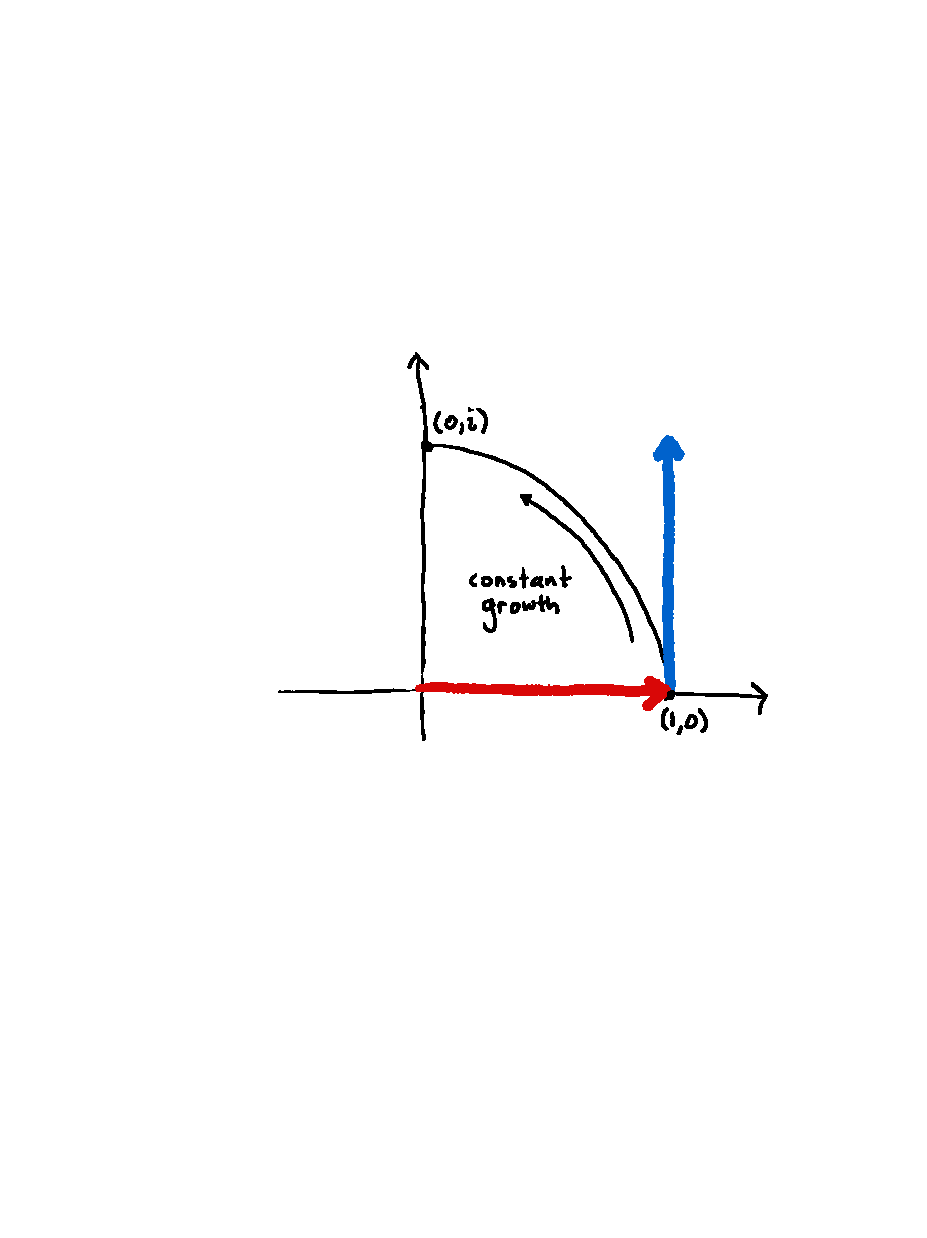
\includegraphics[height=0.9\paperheight]{constant-growth.pdf}	
		\end{figure}
	\end{frame}
	
	\begin{frame}[c]\centering
		it's $e^x$
		
		if we want to represent a point on the complex unit circle by \textbf{scaling} and \textbf{rotation}, we can write this as $$e^{a+bi} = e^a \cdot e^{bi}. $$
		but if we translate our $a+bi$ into \textbf{polar coordinates} with radius $1$, we get $$ e^{1 \cdot i \cdot t} = \underbrace{e^i}_{\mathclap{\text{rotation}}} \cdot e^t $$
	\end{frame}
	
	\begin{frame}[c]
		\begin{figure}
			\centering
			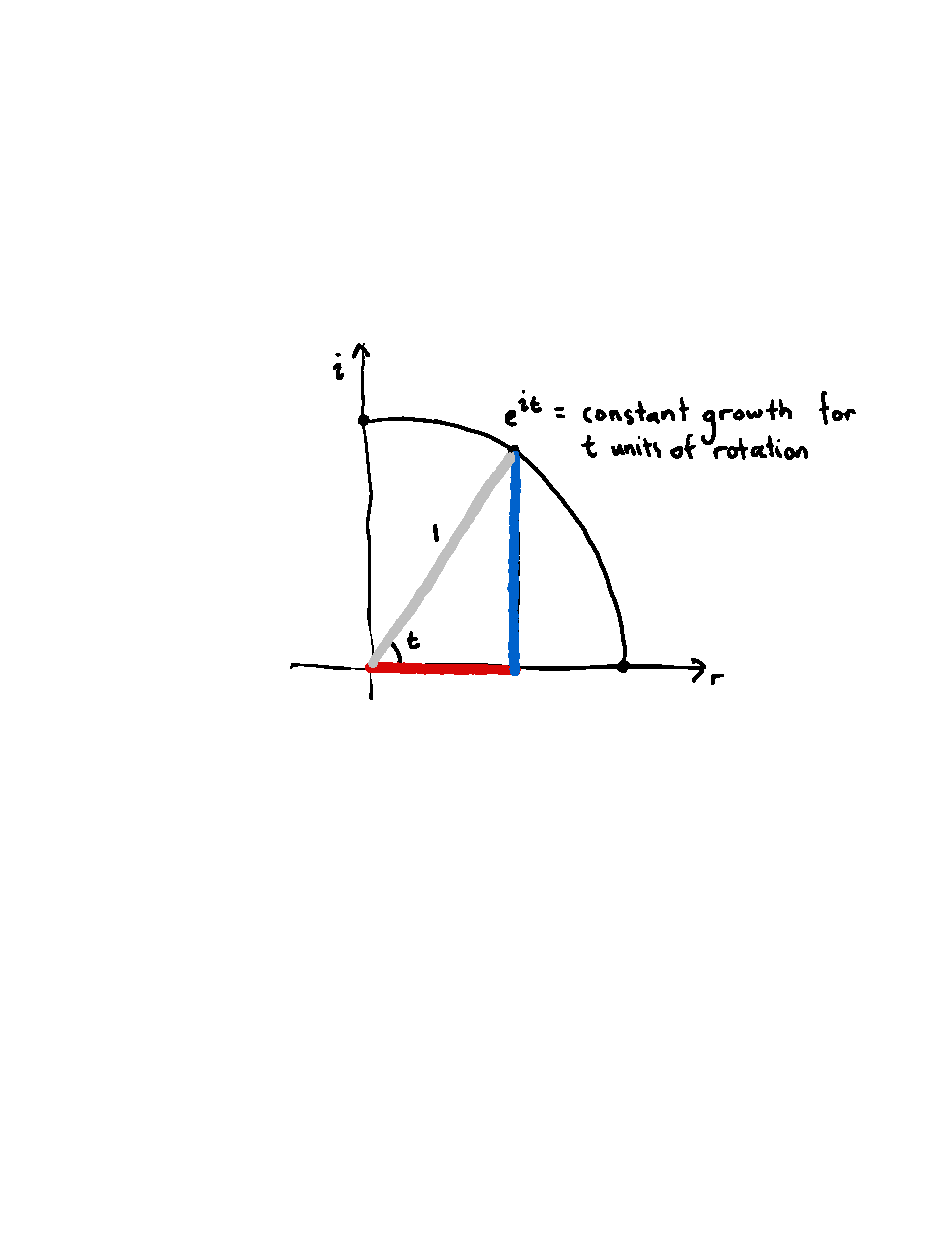
\includegraphics[height=0.9\paperheight]{constant-growth-with-e.pdf}	
		\end{figure}
	\end{frame}
	
	\begin{frame}[c]\centering
		... and because we express polar coordinates in terms of $\sin$ and $\cos$...
	\end{frame}
	
	\begin{frame}[c]
		\begin{figure}
			\centering
			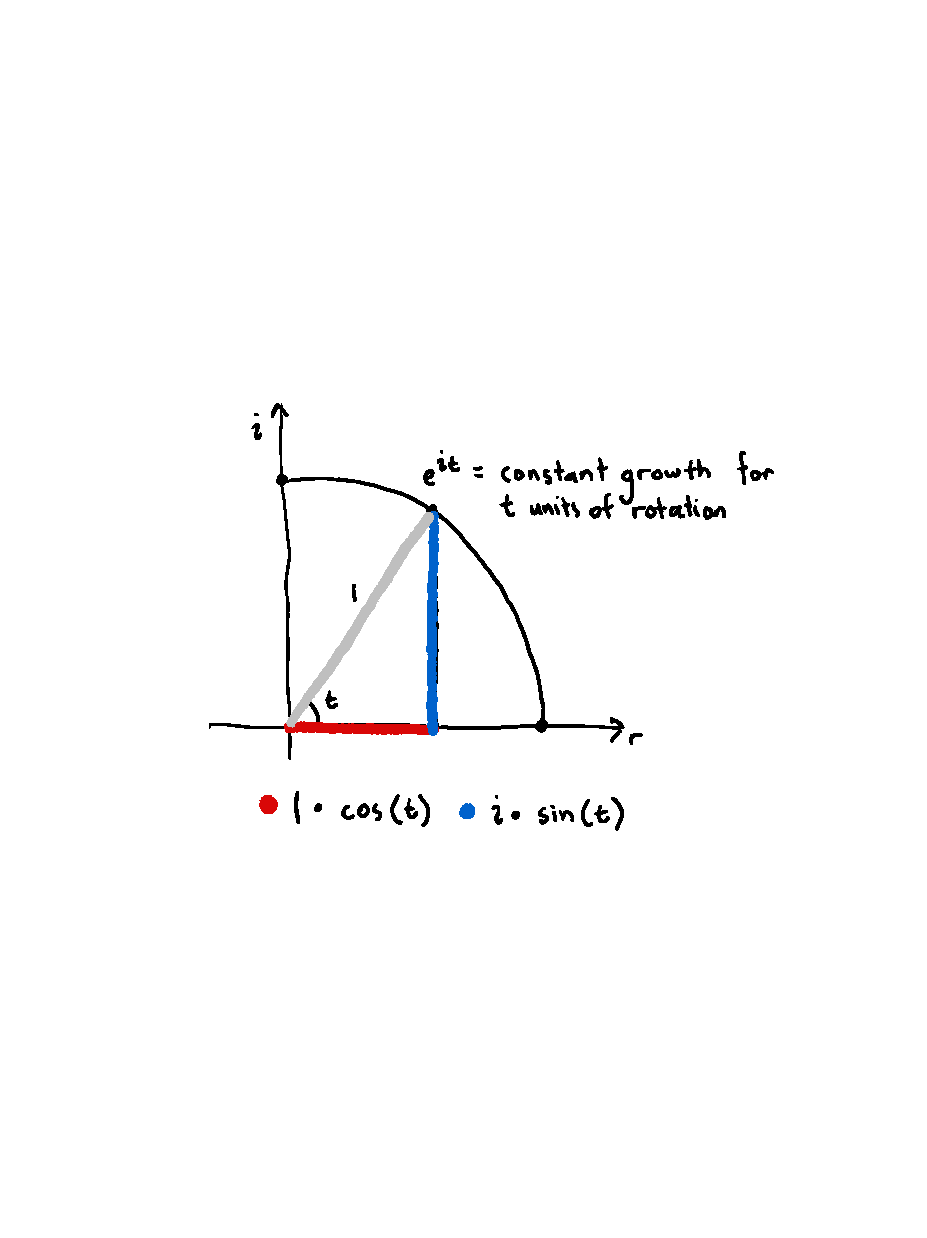
\includegraphics[height=0.9\paperheight]{constant-growth-with-e-with-trig.pdf}
		\end{figure}
	\end{frame}
	
	\begin{frame}[c]\centering
		so our expressions $$ e^{ix} $$ and $$ \cos x + i \sin x $$ represent \textit{the same thing!}
	\end{frame}
	
	\begin{frame}[c]\centering
		the \textit{unit hyperbola} $$ x^2-y^2 =1 $$ is like a circle because it \textbf{grows at precisely the same rate everywhere}, so we can define analogous trig functions on it!
	\end{frame}
	
	\begin{frame}[c]
		\begin{figure}
			\centering
			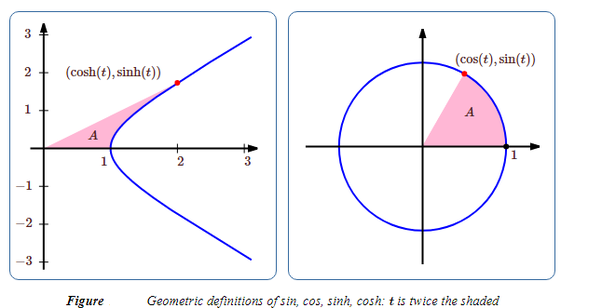
\includegraphics[height=0.9\paperheight]{hyperbola.png}
		\end{figure}
	\end{frame}
	
\end{document}
